\documentclass[../main.tex]{subfiles}
\begin{document}

\chapter{Lecture 21 - 25-05-2020}

\section{Pegasos in Kernel space}

Objective function was $$F_\lambda (w) = \frac{1}{m} \sum_{t=1}^{m} h_t(w) + \frac{1}{2} \|w\|^2 \quad w \in \barra{R}^d$$
$$
w_{T+1} = \frac{1}{\lambda \, T} \sum_{t=1}^T y_{st} \, x_{st} \, I \{ h_{st} (w_t) > 0 \} \qquad s_1, ..., s_t \quad (realised \ draws \ in \ training)
$$
$$
K \qquad H_k = \{ \sum_i \alpha_i k(x_i, \cdot) , \alpha_i, x_i \} \qquad g \in H_k
$$
$$
F_\lambda = \frac{1}{m} \sum_{t=1}^m h_t(g) + \frac{1}{2}
\| g\|^2 \qquad h_t(g) = \left[ 1- y_t \, g(x_t) \, \right]_+ $$
$$
g_{T+1} = \frac{1}{\lambda \, T} \sum_{t=1}^T \red{ y_{st} \, k (x_st, \cdot) \, I \{ h_{st}(g_t) > 0 \} }
$$
where \red{red} part is $v_{st}$
\section{Stability}
A way to bound the risk of a predictor. \\ Controlling the variance error and leave to the user the job to minimise the bias.
\\ Variance error is due to the fact that the predictor an algorithm generate from the training set will depends strongly on the training set itself.
If we perturb the training set our predictor will change a lot.
\\\\
Minimisation of training error $ \Rightarrow $ predictor changes if training set if perturbed. $\Rightarrow $ risk of overfitting 
\\
Stability is the opposite since avoid overfitting when we perturbing the training set.
\\
\begin{itemize}
\item $S$ Training set $(x_t,y_t)...(x_m, y_m)$
\item loss function $\ell$ 
\item distribution $D$
\end{itemize}
$h: X \rightarrow Y$ $\ell_D(h)$ risk of $h$\\
$z_t = (x_t,y_t) \, \ell(h_t, z_t) = \ell(h(x_t),y_t)$
$$
\hat{\ell}_s(h) = \frac{1}{m} \sum_{t=1}^m \ell(h,z_t)
$$
Perturbation $z_t' = (x_t', y_t') $ also drawn from $D$
\\
$
S^{(t)} \textbf{is $S$ where $z_t$ is replaced by $z'_t$  }
$
$h_s= A(S)$
\\
A learning algorithm is $\varepsilon$-stable $\qquad$ $(\varepsilon > 0) \qquad h_s^{(t)} = A(S^{(t)})$
$$
\ell(h_s^{(t)}, z_t) - \ell(h_s, z_t)
$$
we expect this subtraction result to be positive.
$$
\barra{E} \left[ \,\ell(h_s^{(t)}, z_t) - \ell(h_s, z_t) \, \right] \leq \varepsilon \qquad \forall t = 1, ...m 
$$
where $\barra{E}[ \ ] \rightarrow s,z_t'$
\\
$z_t$ and $z'_t$ come from $D$ both
\\
$$
\barra{E} \left[ \ell(h_s,z'_t) - \ell(h_s^{(t)}, z_t' ) \right] \leq \varepsilon
$$
\bred{Theorem}
\\
If $A$ is $\varepsilon$-stable, then $$ 
\barra{E} \left[ \ell_D(h_s) - \hat{\ell}_s(h_s) \right] \leq \varepsilon
$$
\\
Proof: \ $S \qquad z_t = (x_t, y_t) \qquad s' \qquad z'_t = (x_t',y_t') \qquad D$
$$
\barra{E} \left[ \hat{\ell}_s (h_s) \right] = \barra{E} \left[ \frac{1}{m} \sum_{t=1}^m \ell(h_s,z_t) \right] = \frac{1}{m} \sum_{t=1}^m \barra{E} \left[ \ell(h_s, z_t ) \right] \ = \ \frac{1}{m} \sum_{t=1}^m \barra{E} \left[ \ell(h_s^{(t)}, z_t') \right]
$$
$$
\ell_D(h_s) = \barra{E} \left[ \ell(h_s, z'_t) | S \right] = \frac{1}{m} \sum_{t=1}^m \barra{E} \left[ \ell(h_s, z'_t) \right]
$$
Average with respect to random draw of $S$\\
$
\barra{E} \left[ \ell_D (h_s) \right] = \frac{1}{m} \sum_{t=1}^m \barra{E} \left[ \ell(h_s, z'_t)\right]
$
$$
\barra{E} \left[ \ell_D(h_s) - \hat{\ell}_s (h_s) \right] = \frac{1}{m} \sum_{t=1}^m \barra{E} \left[ \ell(h_s, z'_t) - \ell(h_s^{(t)}, z'_t \right] \leq \varepsilon
$$
A stable algorithm is not overfitting (but they still underfit!).
\\So if an $ERM$ algorithm is $\varepsilon$-stable, it would be pretty good.
\\\\
\bred{Theorem}
\\
If \textbf{$A$} is $\varepsilon$-stable and it approximates $ERM$ in a class $H$: 
$$
\hat{\ell}_s \leq \min_{h \in H} \hat{\ell}_s (h) + \gamma \qquad \forall s, \ h_s = A(S)
$$ 
for some $\gamma > 0$, then:
$$
\barra{E} \left[ \ell_D (h_s) \right] \leq \min_{h \in H} \ell_D(h) + \varepsilon + \gamma
$$
\bred{Proof}
\\
$$
\barra{E} \left[ \ell_D(h_s) \right] = \barra{E} \left[ \ell_D (h_s) - \hat{\ell}_s(h_s) \right] + \barra{E} \left[ \hat{\ell}_s(h_s) - \hat{\ell}_s (h^*) \right] + \barra{E} \left[ \ell_s (h^*) \right]
$$
$$
h^* = arg \min_{h \in H} \ \ell_D (h)
$$
$$
\barra{E} \left[ \hat{\ell}(h^*) \right] = \ell_D(h^*) \ \longrightarrow \ \barra{E} \left[ \frac{1}{m} \sum_t \ell(h^*, z_t) \right] = \frac{1}{m} \sum_t \red{\barra{E} \left[ \ell(h^*, z_t ) \right] }
$$
where \bred{red} is $ \ell_D(h^*)$
\\\\
$
\ell(\cdot , z) 
$ is a convex function $\ell(w,z)$ \\ $\exists L > 0 \qquad | \ell(w,z)- \ell(z,z) | \leq L \| w-w'\|$
\\
$z = (x,y)$
\\
In the case of SVM, $\ell(w,z) = \left[ \- y \, w^T \, x \right]_+$
$ \exists L > 0 \quad \forall z \ \forall w, w'$ 
$$
| \ell(w,z) - \ell(w',z) | \leq L \| w-w'\|
$$
where $ell$ is \textbf{Lipschitz}
\\\\
\bred{Theorem}
\\
Let $\ell$ be convex, Lipschitz and differentiable.
\\
Consider $A$ \qquad $ A(S) = w_s$ where 
\\
$$
w_s = arg \min_{w \in \barra{R}^d} \left( \hat{\ell}_s (w) + \frac{\lambda}{2}\| w\|^2 \right)
$$
If $\ell$ is hinge loss, then $A$ is $SVM$.\\
then $A$ is $\frac{(2 \, L)^2}{\lambda \, m}$-stable \qquad $\forall \lambda > 0 $
\\\\
\bred{Proof}
\\
Fix $\lambda > 0$ \qquad $F_s (w) = \hat{\ell}_s(w) + \frac{\lambda}{2} \| w \|^2$
$$
w_s = arg \min_{w \in \barra{R}^d} F_s (w) \qquad w_s^{(t)} = arg \min_{w \in \barra{R}^d } F_s^{(t)}(w)
$$
$$
\ell(w_s,z'_t) - \ell(w_s^{(t)},z'_t) \leq \varepsilon \qquad \forall s, z'_t \ \forall t 
$$
Use Lipschtiz
$$
| \ell(w_s, z'_t) - \ell(w_s^{(t)}, z'_t) | \leq L \| w_s-w_s^{(t)} \|
$$
$w = w_s, \ w' = w_s^{(t)}$
$$
F_s(w') - F_s(w) = \hat{\ell}(w') - \hat{\ell}(w) + \frac{1}{2} \| w' \|^2 - \frac{\lambda}{2} \|w \|^2 \ =
$$
$$
\ = \
 \hat{\ell}_s^{(t)}(w') - \hat{\ell}_s^{(t)} + \frac{1}{m} \left( \ell(w', z_t) - \ell(w,z_t) \right) - \frac{1}{m} \left( \ell(w', z'_t ) - \ell(w, z'_t) \right) + \frac{\lambda}{2} ( \| w'\|^2 - \| w \|^2 ) \ =
$$
$$
= \ \red{F_s^{(t)} (w') - F_S^{(t)}(w)} + \frac{1}{m} (\ell(w', z_t) - \ell (w,z_t) ) - \frac{1}{m}( \ell(w',z'_t)-\ell(w,z'_t)) \ \leq
$$
where \bred{red} is $\leq 0$
$$
\ \leq \ |\frac{1}{m}\ell(w',z_t) - \ell(w, z_t) | + \frac{1}{m} | \ell(w',z_t') - \ell(w, z'_t) | \leq \
$$
  ----- MANCAAAAAAA ----
$$
F_s(w) - F_s(w') \leq \frac{2 \, L}{m} \| w- w'\|
$$
$F_s$ is $\lambda$-SC \qquad $F_s(w') \geq F_s(w) + \nabla F_s(w)^T (w'-w)+\frac{\lambda}{2}\|w- w'\|^2$
Since $w$ is minimiser of $F_s$ the gradiant $ \nabla F_s(w)^T = 0$
Therefore:
$$
F_s(w') - F_s(w) \geq \frac{1}{2}
 \| w- w'\|^2 $$
$$
\frac{\lambda}{2} \| w- w'\|^2 \geq \frac{2 \, L}{m} \|w-w'\| \Rightarrow \| w-w' \| \leq \frac{4 \, L}{\lambda \, m} 
$$
$$
\ell(w_s, z'_t) - \ell(w_s^{(t)}, z'_t) \leq \frac{4 \, L^2}{\lambda \, m}
$$
We now know the stability of the SVM.
\begin{figure}[h]
    \centering
    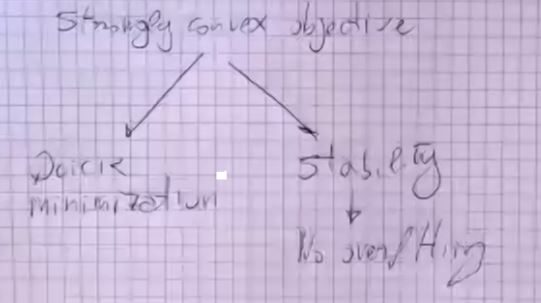
\includegraphics[width=0.8\linewidth]{../img/lez21-img1.JPG}
    \caption{}
    %\label{fig:}
\end{figure}
\end{document}
